\documentclass[conference]{IEEEtran}
\IEEEoverridecommandlockouts
\usepackage{cite}
\usepackage{amsmath,amssymb,amsfonts}
\usepackage{graphicx}
\usepackage{textcomp}
\usepackage{xcolor}
\usepackage{makecell}
\usepackage{subcaption}
\usepackage{tikz}
\usepackage{circuitikz}
\usetikzlibrary{arrows.meta, positioning, calc}
\ctikzset{american}

\def\BibTeX{{\rm B\kern-.05em{\sc i\kern-.025em b}\kern-.08em
    T\kern-.1667em\lower.7ex\hbox{E}\kern-.125emX}}

\begin{document}

\title{Equivalent Circuit Models of Near-Field Coupling between Electrically Small Antennas and TEM Cells}

\author{%
\IEEEauthorblockN{Simon Prato}
\IEEEauthorblockA{\textit{\makecell{Institute of Fundamentals and Theory\\ in Electrical Engineering}} \\
\textit{Graz University of Technology}\\
Graz, Austria \\
simon.prato@student.tugraz.at}
\and
\IEEEauthorblockN{Dominik Kreindl}
\IEEEauthorblockA{\textit{\makecell{Institute of Fundamentals and Theory\\ in Electrical Engineering}} \\
\textit{Graz University of Technology}\\
Graz, Austria \\
dominik.kreindl@student.tugraz.at}
\and
\IEEEauthorblockN{Thomas Bauernfeind}
\IEEEauthorblockA{\textit{\makecell{Institute of Fundamentals and Theory\\ in Electrical Engineering}} \\
\textit{Graz University of Technology}\\
Graz, Austria \\
t.bauernfeind@tugraz.at}
}

\maketitle

\begin{abstract}
Light sources in optical sensor packages of integrated circuits (ICs) require apertures for light transmission and, therefore, cannot be effectively shielded from electromagnetic waves. Furthermore, bond wires are implemented, which form electrically small structures that emit unwanted radiation and thereby behave as antennas. Transverse-electromagnetic (TEM) cells are standardized environments for characterizing these emissions. 
This paper develops equivalent circuit models (EQCs) for the near-field coupling between electrically small antennas and a TEM cell. Lumped elements effectively model such antennas and their coupling paths due to their small size in comparison to the wavelength. The EQC component values are extracted from finite element method (FEM) simulations. The coupling behavior described by the EQC are compared with that from FEM simulations of the TEM cell, demonstrating good agreement and confirming that the proposed models correctly represent both the electric and magnetic coupling mechanisms.
\end{abstract}

\begin{IEEEkeywords}
Electromagnetic Compatibility, TEM Cell, Equivalent Circuit Model,
Dipole Moments, Near-Field Coupling, Electrically Small Antenna.
\end{IEEEkeywords}

\section{Introduction}




A bonding wire is typically required to connect the semiconductor chip
to its package in order to route signals to the surrounding circuit.
Because of their geometry, bond wires inevitably form current loops that
cause unwanted electromagnetic interference (EMI) radiation at fast signal
rise times. A straightforward remedy is to surround the device with
electrically conductive shielding~\cite{b1}. However, this approach is
inapplicable to optical sensor ICs that incorporate vertical-cavity
surface-emitting lasers (VCSELs)~\cite{b2}: the optical apertures required
for light emission and reception prevent a complete metallic enclosure.

An alternative strategy is to characterize the parasitic radiators by their
dipole moments and to exploit geometric cancellation effects at the bond-wire
level. This requires a fundamental understanding of how electrically short
structures couple to the IC stripline test environment~\cite{b5}. Because the
IC stripline operates on the same TEM wave-propagation principle as a generic
TEM cell~\cite{b3}, a rectangular TEM cell is used as a computationally
tractable surrogate for initial FEM investigations.

Since bond-wire dimensions are small compared to the free-space wavelength up
to 3\,GHz, these structures are electrically short and can be fully
characterized by an electric dipole moment $\mathbf{m}_e$ and a magnetic
dipole moment $\mathbf{m}_m$. Replacing the antenna by its dipole moments and
modelling the coupling to the TEM cell with lumped elements yields an
equivalent circuit model (EQC) that provides direct physical insight into the
coupling mechanisms and runs orders of magnitude faster than a full-wave FEM
simulation.

This paper derives EQCs for two representative test structures---a monopole
antenna (dominant capacitive coupling) and a gapped-loop antenna (combined
capacitive and inductive coupling)---and validates the predicted dipole moments
against full-wave TEM cell FEM simulations.

\section{TEM Cell Measurement and Dipole Moment Extraction}

The TEM cell~\cite{b3} provides a controlled propagation environment for
characterizing IC emission. As shown in Fig.~\ref{fig:stripline}, the device
under test (DUT) is placed between the septum and the cell enclosure. The
septum acts as the inner conductor of a coaxial-like transmission line with
wave impedance $Z_W = 50\,\Omega$. A vector network analyzer (VNA) records the
terminal voltages $U_1$ and $U_2$ at the two output ports.

\begin{figure}[t]
  \centerline{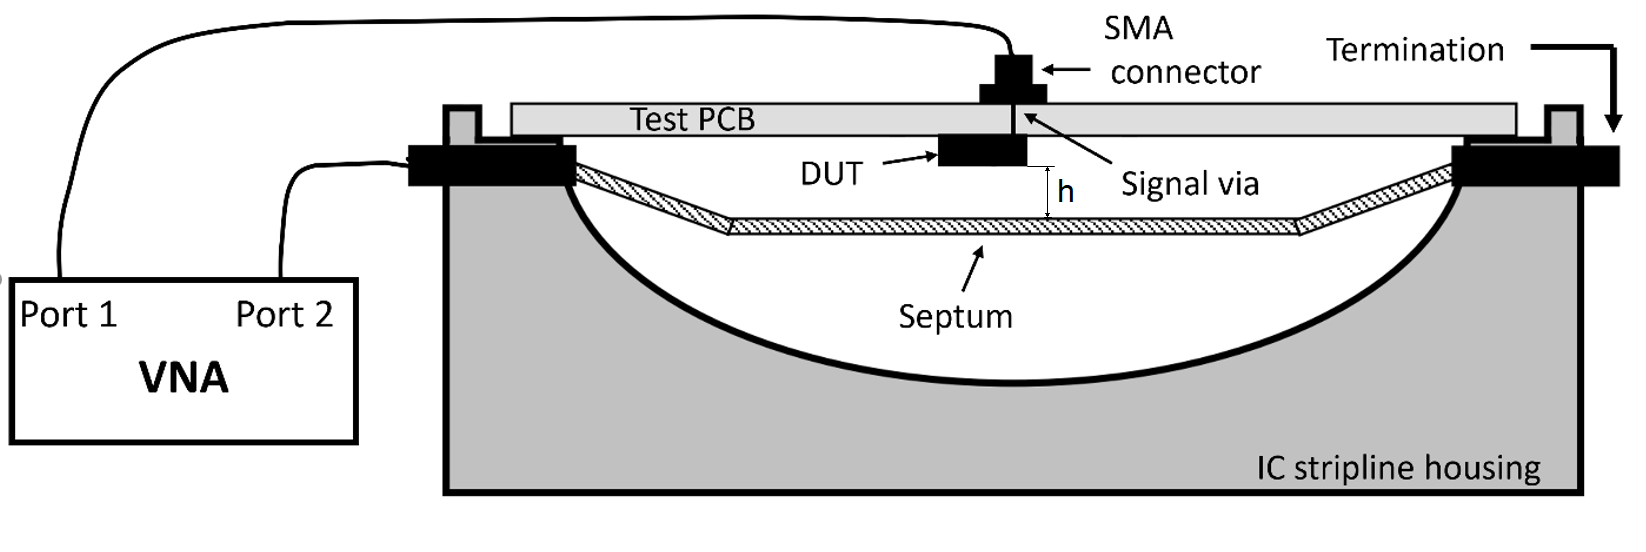
\includegraphics[width=0.48\textwidth]{figures/s12_meas_1.png}}
  \caption{Cross-sectional view of the TEM cell connected to a VNA.
    The parameter $h$ is the distance from the septum to the DUT.}
  \label{fig:stripline}
\end{figure}

For electrically short DUTs the effective electric and magnetic dipole moments
can be extracted directly from the port voltages~\cite{b6}:
\begin{equation}
  |m_e| = \frac{|U_1 + U_2|\,h}{Z_W}, \label{eq:me}
\end{equation}
\begin{equation}
  |m_m| = \frac{|U_1 - U_2|\,h\,Z_0}{Z_W}, \label{eq:mm}
\end{equation}
where $h$ is the septum--DUT distance, $Z_W = 50\,\Omega$, and
$Z_0 = 377\,\Omega$ is the free-space wave impedance. The sum
$U_1\!+\!U_2$ is sensitive to the TEM mode driven by the electric dipole,
while the difference $U_1\!-\!U_2$ isolates the magnetic dipole contribution.

\section{Equivalent Circuit Models and Results}

\subsection{Antenna Model and Parameter Extraction}

Because both test structures are electrically short, their impedance behaviour
can be captured by a reduced RLC circuit. For the \emph{monopole} antenna the
dominant reactive element at low frequencies is the capacitance $C_A$,
representing the energy stored in the electric near field~\cite{Chu1948}; $L_A$
accounts for the stored magnetic energy and $R_A$ for radiation losses. For the
\emph{gapped-loop} antenna the same topology applies but with predominantly
inductive character~\cite{Balanis1997}; ohmic loss and internal inductance are
neglected by modelling the antenna as a perfect electric conductor.

The parameters $L_A$ and $C_A$ are extracted from free-space FEM simulations
via the stored-energy relations
\begin{equation}
  L_A = \frac{2W_m}{I_{L_A}^2}, \qquad C_A = \frac{2W_c}{V_{C_A}^2},
  \label{eq:params}
\end{equation}
where $W_m$ ($W_c$) is the magnetic (electric) stored energy. This gives
$C_A = 98.4\,\text{fF}$, $L_A = 1.14\,\text{nH}$ for the monopole and
$C_A = 38.2\,\text{fF}$, $L_A = 2.14\,\text{nH}$ for the gapped loop.

\subsection{Extended Circuit Including TEM Cell Coupling}

The antenna EQC is extended to include the TEM cell, modelled by a symmetric
inductance $L_T\!=\!L_{T1}\!+\!L_{T2}$ and capacitance
$C_T\!=\!C_{T1}\!+\!C_{T2}$. Two coupling elements complete the model:
(i)~a coupling capacitance $C_k$ that injects displacement current from the
antenna into the TEM cell, driving $m_e$; and
(ii)~mutual inductances $M_{A,T1}$ and $M_{A,T2}$ between $L_A$ and the
septum inductances $L_{T1}$, $L_{T2}$, driving $m_m$ via inductive voltage
injection. Figs.~\ref{fig:eqc_monopole} and~\ref{fig:eqc_loop} show the
resulting circuits for the monopole ($M\!\approx\!0$,
$C_k\!\approx\!1.68\,\text{pF}$) and the gapped-loop (both $C_k$ and $M$
non-negligible), respectively.

% ---- EQC MONOPOLE (circuitikz) ----
\begin{figure}[t]
\centering
\resizebox{\columnwidth}{!}{%
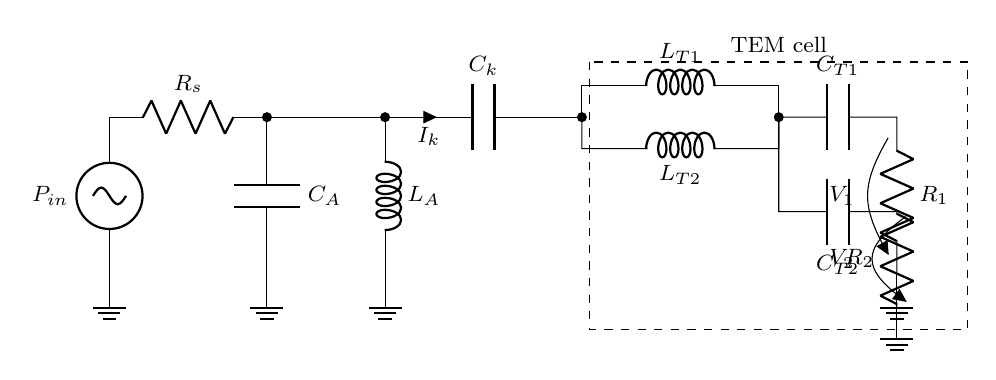
\begin{tikzpicture}[
  every node/.style={font=\footnotesize},
  N/.style={circle,draw,inner sep=2pt}]
  % Source + Rs
  \draw (0,0) to[sV, l=$P_{in}$] (0,2)
              to[R,  l=$R_s$]     (2,2);
  \draw (0,0) node[ground]{};
  % C_A shunt to ground
  \draw (2,2) to[C, l=$C_A$] (2,0) node[ground]{};
  % junction A
  \node[circ] at (2,2){};
  % L_A shunt to ground
  \draw (2,2) -- (3.5,2) to[L, l=$L_A$] (3.5,0) node[ground]{};
  % C_k in series
  \draw (3.5,2) to[C, l=$C_k$, i>_=$I_k$] (6,2);
  \node[circ] at (3.5,2){};
  % TEM cell bracket label
  \draw[dashed] (6.1,2.7) rectangle (10.9,-0.7);
  \node[above] at (8.5,2.7) {TEM cell};
  % Split: L_T1 top, L_T2 bottom
  \draw (6,2) -- (6,2.4) to[L, l=$L_{T1}$] (8.5,2.4) -- (8.5,2);
  \draw (6,2) -- (6,1.6) to[L, l_=$L_{T2}$] (8.5,1.6) -- (8.5,2);
  \node[circ] at (6,2){};  \node[circ] at (8.5,2){};
  % C_T1, R_1
  \draw (8.5,2) to[C, l=$C_{T1}$] (10,2)
                to[R, l=$R_1$, v=$V_1$] (10,0) node[ground]{};
  % C_T2, R_2
  \draw (8.5,2) -- (8.5,0.8) to[C, l_=$C_{T2}$] (10,0.8)
                to[R, l_=$R_2$, v_=$V_2$] (10,-0.4) node[ground]{};
\end{tikzpicture}
}
\caption{Extended EQC for the monopole antenna. Mutual inductances vanish
  ($M\!=\!0$); coupling is purely capacitive via $C_k\!\approx\!1.68\,\text{pF}$.}
\label{fig:eqc_monopole}
\end{figure}

% ---- EQC LOOP (circuitikz) ----
\begin{figure}[t]
\centering
\resizebox{\columnwidth}{!}{%
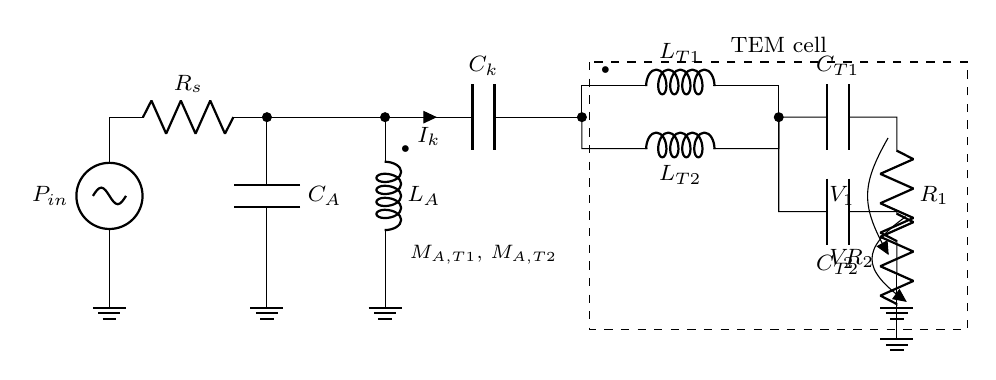
\begin{tikzpicture}[
  every node/.style={font=\footnotesize}]
  % Source + Rs
  \draw (0,0) to[sV, l=$P_{in}$] (0,2)
              to[R,  l=$R_s$]     (2,2);
  \draw (0,0) node[ground]{};
  % C_A shunt
  \draw (2,2) to[C, l=$C_A$] (2,0) node[ground]{};
  \node[circ] at (2,2){};
  % L_A shunt (with coupling dots)
  \draw (2,2) -- (3.5,2)
              to[L, l=$L_A$, name=LA] (3.5,0) node[ground]{};
  \node[circ] at (3.5,2){};
  \node[right=2pt, font=\tiny] at (3.5,1.6) {$\bullet$};
  % C_k
  \draw (3.5,2) to[C, l=$C_k$, i>_=$I_k$] (6,2);
  % Coupling note
  \node[below, font=\scriptsize] at (4.75,0.5)
    {$M_{A,T1},\,M_{A,T2}$};
  % TEM cell box
  \draw[dashed] (6.1,2.7) rectangle (10.9,-0.7);
  \node[above] at (8.5,2.7) {TEM cell};
  % L_T1 top (dot for polarity)
  \draw (6,2) -- (6,2.4) to[L, l=$L_{T1}$, name=LT1] (8.5,2.4) -- (8.5,2);
  \node[above=1pt, font=\tiny] at (6.3,2.4) {$\bullet$};
  % L_T2 bottom (dot opposite polarity)
  \draw (6,2) -- (6,1.6) to[L, l_=$L_{T2}$, name=LT2] (8.5,1.6) -- (8.5,2);
  \node[circ] at (6,2){};  \node[circ] at (8.5,2){};
  % C_T1, R_1
  \draw (8.5,2) to[C, l=$C_{T1}$] (10,2)
                to[R, l=$R_1$, v=$V_1$] (10,0) node[ground]{};
  % C_T2, R_2
  \draw (8.5,2) -- (8.5,0.8) to[C, l_=$C_{T2}$] (10,0.8)
                to[R, l_=$R_2$, v_=$V_2$] (10,-0.4) node[ground]{};
\end{tikzpicture}
}
\caption{Extended EQC for the gapped-loop antenna. Both $C_k$ (electric) and
  $M_{A,T1/2}$ (magnetic) coupling paths are active.
  $C_A\!=\!38.2\,\text{fF}$, $L_A\!=\!2.14\,\text{nH}$.}
\label{fig:eqc_loop}
\end{figure}

\subsection{Dipole Moment Extraction from the EQC}

The output voltages at $R_1$ and $R_2$ are decomposed by superposition into
a magnetic part $V'_{1,2}$ (driven by $M$) and an electric part $V''_{1,2}$
(driven by $C_k$):
\begin{subequations}\label{eq:voltages}
\begin{align}
  V'_{1,2} &= \pm j\omega M I_{L_A}
    \frac{R_{1,2} \| \tfrac{1}{j\omega C_{T1,2}}}
         {R_{1,2} \| \tfrac{1}{j\omega C_{T1,2}} + j\omega L_{T1,2}},
  \label{eq:Vprime}\\
  V''_{1,2} &= \frac{I_k}{2}
    \frac{1/R_{1,2}}{1/R_{1,2} + j\omega C_{T1,2}}.
  \label{eq:Vdprime}
\end{align}
\end{subequations}
The total output is $V_{1,2} = V'_{1,2} + V''_{1,2}$. The modal wave
amplitudes $a_\mathrm{TEM}\!=\!\sqrt{V_1^2/R_1}$ and
$b_\mathrm{TEM}\!=\!\sqrt{V_2^2/R_2}$ are then inserted into
\eqref{eq:me}--\eqref{eq:mm} to obtain the EQC dipole moments.
The \emph{phase difference} between $m_e$ and $m_m$ is the primary
indicator for the relative balance of the two coupling mechanisms.

\subsection{Results: FEM vs.\ EQC Comparison}

Fig.~\ref{fig:test_loop} shows the gapped-loop test structure. The small air
gap produces a pronounced electric dipole moment in addition to the magnetic
dipole from the current loop. Fig.~\ref{fig:loop_results} shows the dipole
moments obtained from full-wave TEM cell FEM simulations. The electric dipole
moment rises linearly with frequency---a signature absent in a closed loop---
while the magnetic dipole moment is roughly constant over the investigated
range.

\begin{figure}[t]
  \centerline{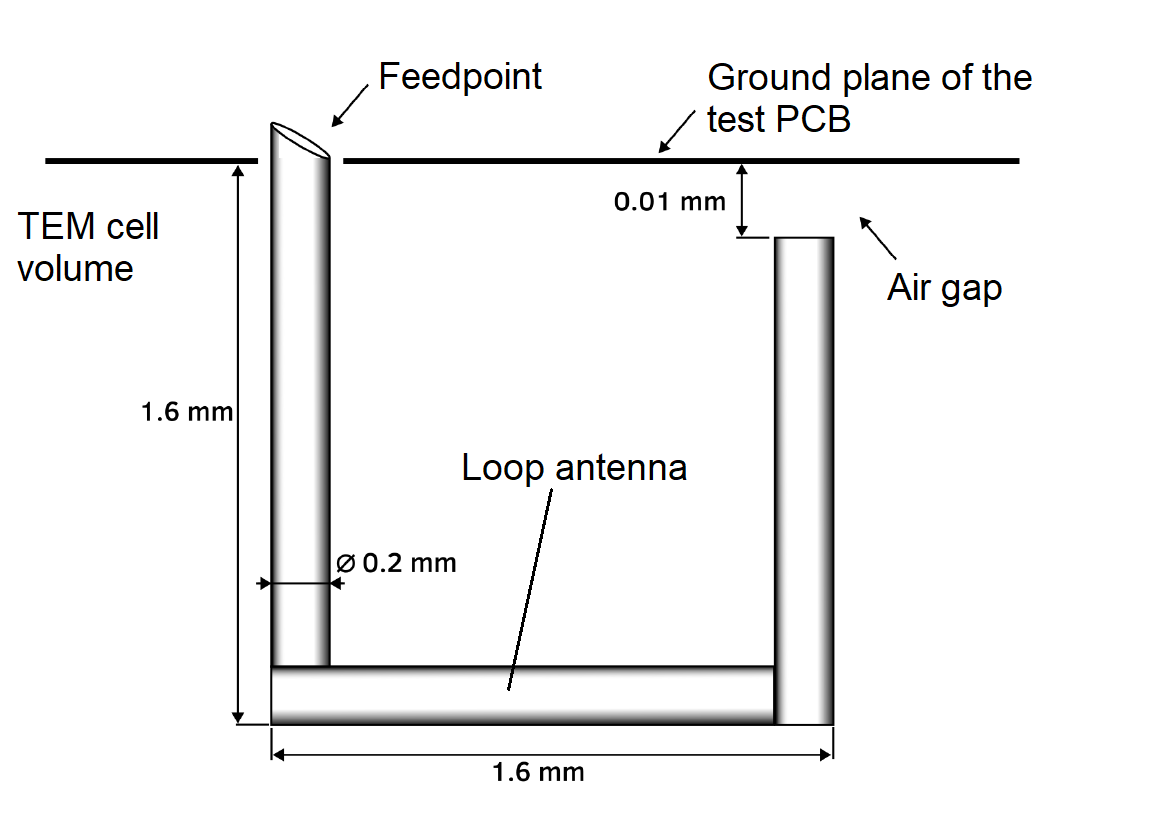
\includegraphics[width=0.36\textwidth]{figures/test_loop.png}}
  \caption{Gapped rectangular loop test structure. The current loop produces
    $\mathbf{m}_m$; the air gap adds $\mathbf{m}_e$.}
  \label{fig:test_loop}
\end{figure}

\begin{figure}[t]
  \centerline{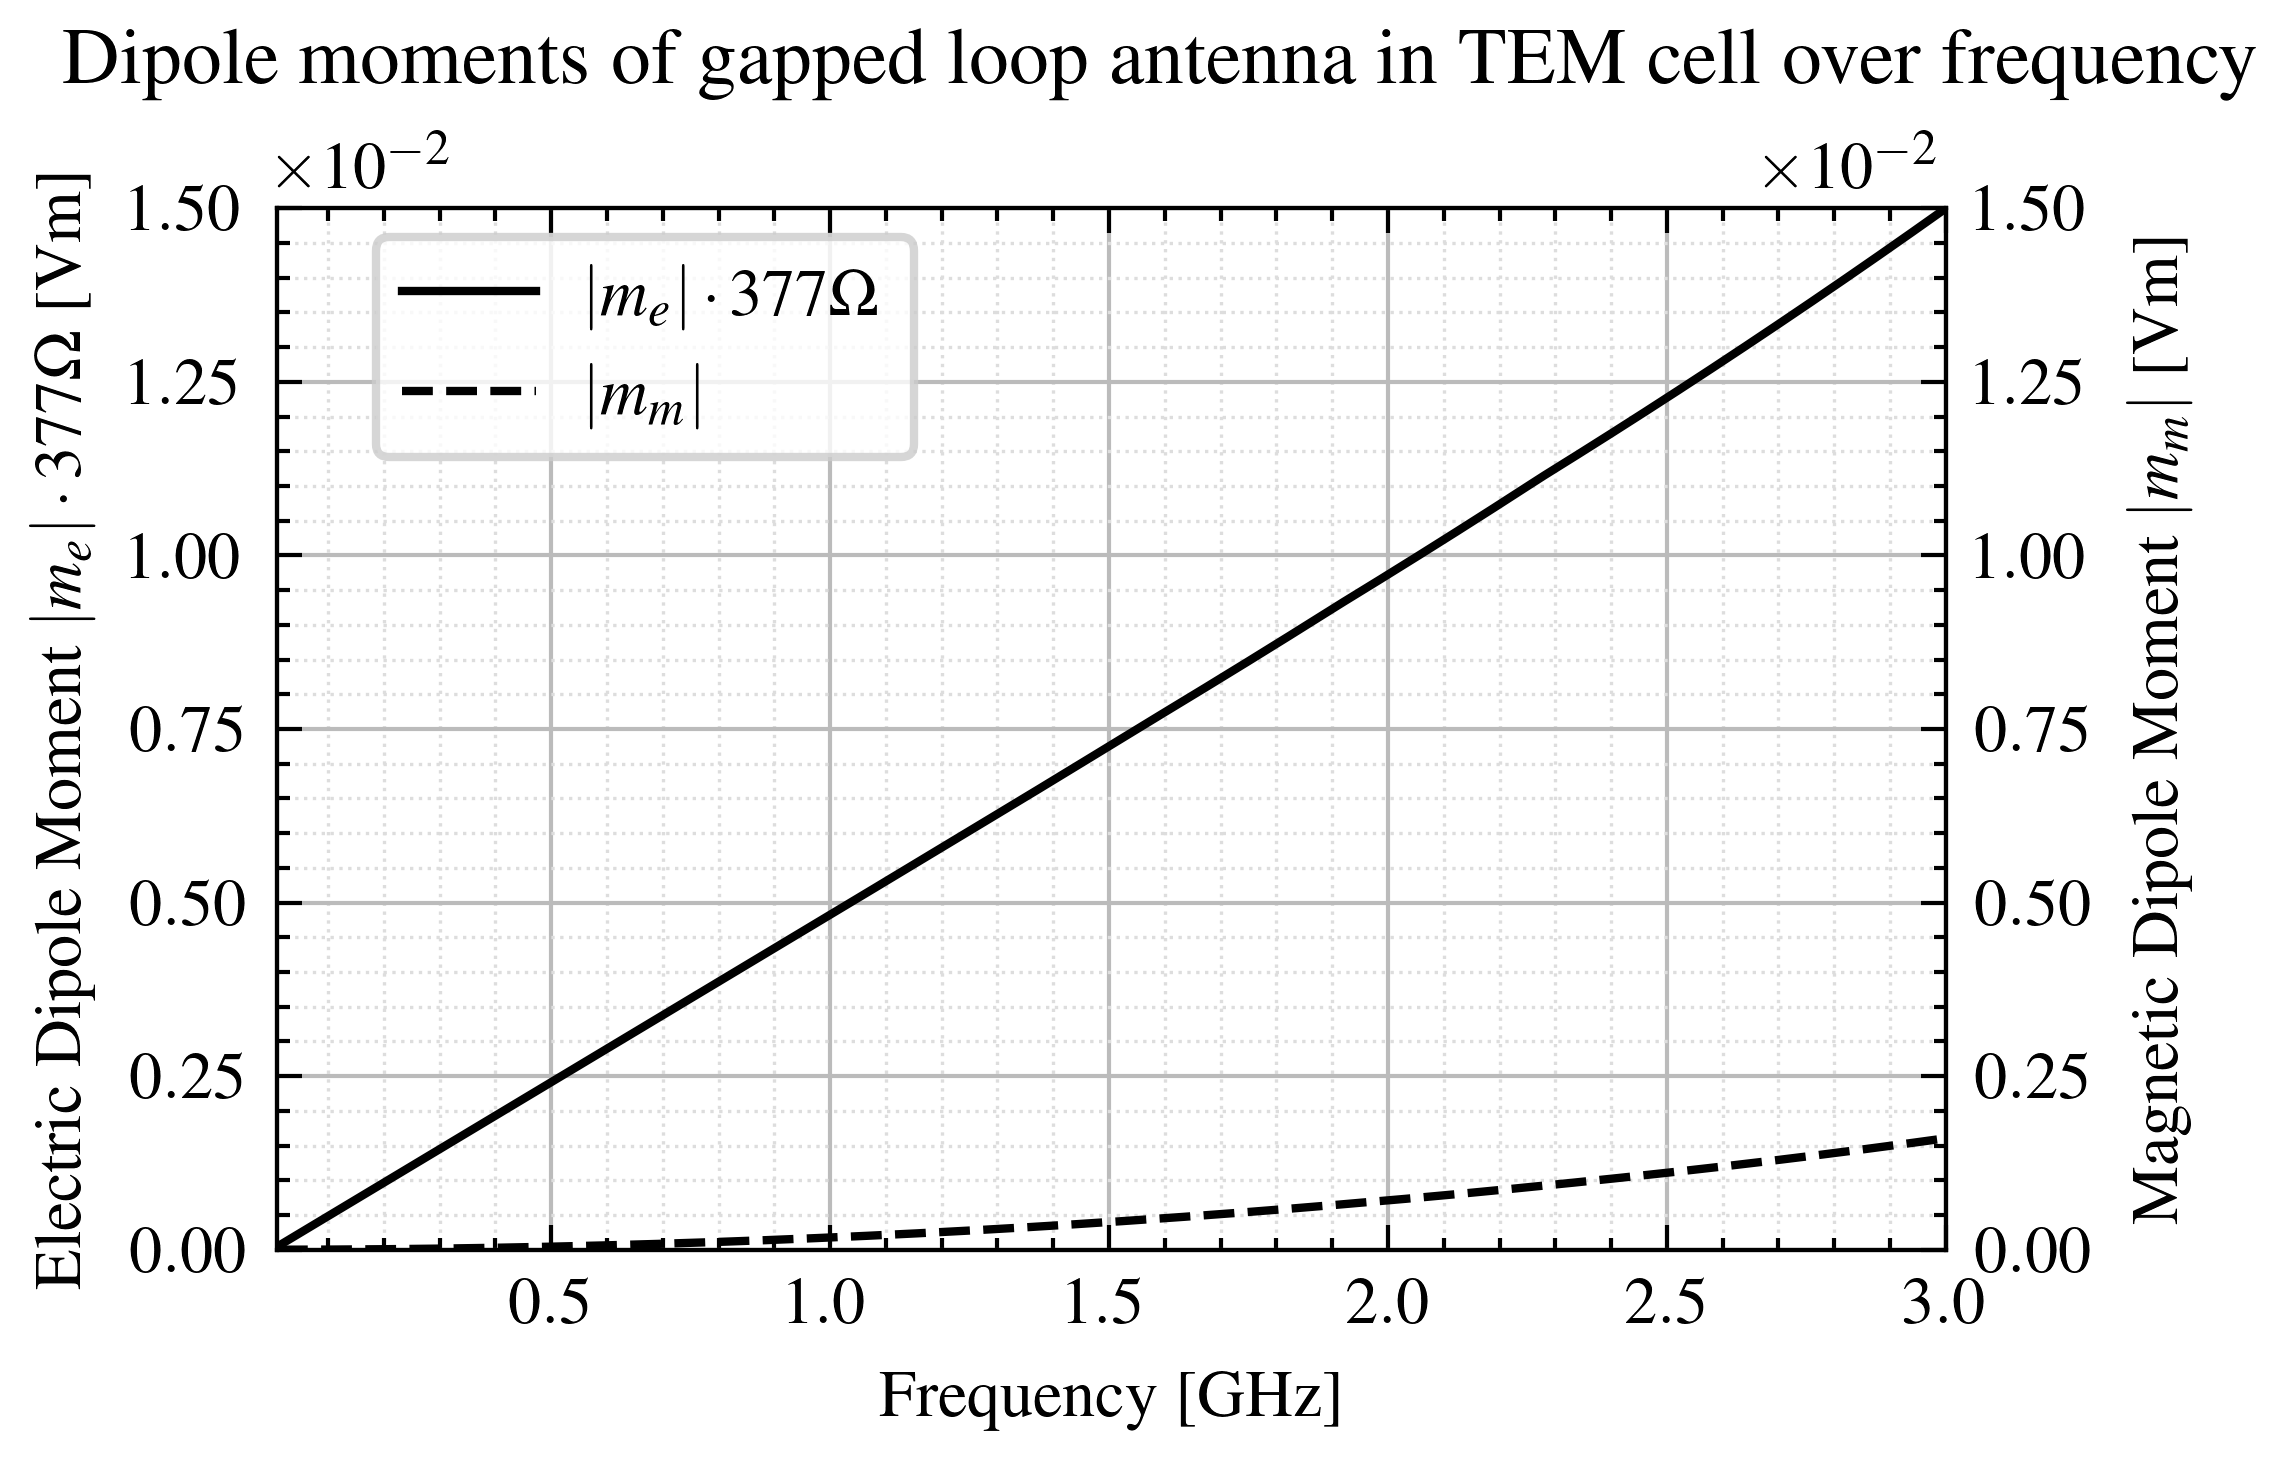
\includegraphics[width=0.46\textwidth]{figures/gapped_loop_moments_corr.png}}
  \caption{Electric and magnetic dipole moments of the gapped-loop antenna
    vs.\ frequency (FEM). $m_e$ is scaled by $Z_0$ for comparison.}
  \label{fig:loop_results}
\end{figure}

The EQC reproduces the linear rise of $m_e$ and the magnitude of $m_m$ in the
upper portion of the frequency range. Deviations at low frequencies are
attributed to numerical sensitivities in the FEM energy extraction at small
field amplitudes, where the extracted $L_A$ and $C_A$ are most sensitive to
meshing errors. For the monopole, only $m_e$ is predicted ($M\!=\!0$) and the
EQC result agrees well with the FEM reference across the full frequency range.

\section{Conclusion}

Lumped-element equivalent circuit models have been developed for the capacitive
and inductive near-field coupling of electrically short antennas to a TEM cell.
The EQC parameters ($C_A$, $L_A$, $C_k$, $M_{A,T}$) are extracted from
free-space FEM energy integrals and are therefore independent of the TEM cell
geometry. Dipole moments predicted by the EQC agree well with full-wave FEM
results for both a monopole (pure capacitive coupling) and a gapped-loop antenna
(combined capacitive and inductive coupling). The phase difference between
$m_e$ and $m_m$ directly reveals the balance between the two coupling mechanisms,
providing physical insight not accessible from full-wave simulation alone. Future
work will apply this methodology to IC bond-wire geometries within the
standardized IC stripline test~\cite{b5}.

\begin{thebibliography}{00}
\bibitem{b1}
B. Conley et al., ``Shielding Methods for Gigahertz-Frequency Wideband
Analog-Integrated Circuits,'' \textit{IEEE Trans. Electromagn. Compat.},
vol.~58, no.~4, pp.~1041--1051, 2016.

\bibitem{b2}
D. Kreindl, B. Weiss, C. Stockreiter, T. Bauernfeind, M. Kaltenbacher,
and M. Faccinelli, ``Measurement and Simulation Methodology for
Characterizing the Shielding Effectiveness of Coating Materials for
Optical Sensors,'' \textit{2023 Int. Symp. Electromagn. Compat.--EMC
Europe}, pp.~1--6, 2023.

\bibitem{b3}
T. Ostermann and B. Deutschmann, ``TEM-Cell and Surface Scan to Identify
the Electromagnetic Emission of Integrated Circuits,'' \textit{Proc.
13th ACM Great Lakes Symp. VLSI}, pp.~76--79, 2003.

\bibitem{b5}
\textit{IEC~61967-8: Integrated Circuits---Measurement of Electromagnetic
Emissions---Part~8: IC Stripline Method.} IEC, Geneva, 2013.

\bibitem{b6}
A. Boyer and S. Ben Dhia, ``Low-Cost Broadband Electronic Coupler for
Estimation of Radiated Emission of ICs in TEM Cell,''
\textit{IEEE Trans. Electromagn. Compat.}, vol.~63, no.~2,
pp.~636--639, 2020.

\bibitem{Chu1948}
L. J. Chu, ``Physical Limitations of Omni-Directional Antennas,''
\textit{J. Appl. Phys.}, vol.~19, no.~12, pp.~1163--1175, 1948.

\bibitem{Balanis1997}
C. A. Balanis, \textit{Antenna Theory: Analysis and Design}, 2nd~ed.,
New York: Wiley, 1997, p.~244.

\bibitem{Pozar2012}
D. M. Pozar, \textit{Microwave Engineering}, 4th~ed.,
New York: Wiley, 2012, p.~175.
\end{thebibliography}

\end{document}
